% MenuNorm — conference working paper
% Build: xelatex menunorm.tex (run twice)
\documentclass[10pt,twocolumn]{article}

\usepackage[a4paper,top=2.3cm,bottom=2.5cm,left=1.9cm,right=1.9cm,columnsep=0.75cm]{geometry}
\usepackage{fontspec}
\usepackage{xeCJK}
\setmainfont{Noto Serif CJK KR}
\setsansfont{Noto Sans CJK KR}
\setmonofont{Noto Sans Mono CJK KR}
\setCJKmainfont{Noto Serif CJK KR}
\setCJKsansfont{Noto Sans CJK KR}
\setCJKmonofont{Noto Sans Mono CJK KR}

\usepackage{graphicx}
\usepackage{booktabs}
\usepackage{amsmath}
\usepackage{caption}
\captionsetup{font=small,labelfont=bf,skip=4pt}
\usepackage{enumitem}
\setlist{nosep,leftmargin=1.2em}
\usepackage[hidelinks]{hyperref}
\usepackage{url}
\urlstyle{same}

\setlength{\parskip}{0pt}
\setlength{\parindent}{1em}

\newcommand{\menunorm}{\textsc{MenuNorm}}
\newcommand{\unmatched}{\texttt{UNMATCHED}}

\begin{document}

\twocolumn[{%
\begin{center}
{\LARGE\bfseries \menunorm{}: Two-Level Standardization of Noisy Korean Product Names\\[2pt]
with Dual-Segmentation Fusion and Guaranteed Category Coverage\par}
\vspace{14pt}
{\large Minyoung Park}\\[2pt]
{\small Department of Computer Science, Gyeongsang National University \;·\; Dream2Real\\
\texttt{github.com/pmy02/Menunorm}}
\vspace{14pt}
\end{center}
\begin{center}
\begin{minipage}{0.92\textwidth}
\small
\textbf{Abstract.}
User-generated Korean product names are noisy: decorations
(\mbox{★짜장면★}), option suffixes (세트, 곱빼기), spacing errors,
Korean--English code-switching (\mbox{cheese돈가스}), and spelling variants
inflate a small menu vocabulary into millions of surface forms. We present
\menunorm{}, a reproducible pipeline that standardizes such names at two
levels: a fine-grained \emph{canonical label} (136 classes) assigned with an
abstention option, and a coarse \emph{delivery-app category} (13 classes)
assigned with \emph{guaranteed full coverage} through a fallback chain. The
matcher fuses two segmentations---a morphological path (MeCab with an
auto-compiled domain user dictionary) and a surface path---by taking the
per-row maximum of character $n$-gram TF--IDF scores, which we show
dominates either path alone. Because the motivating industrial dataset
($\sim$20M records) is under NDA, we release a deterministic synthetic
benchmark whose noise model reproduces the documented real-world corruption
modes, whose class mix is calibrated to published demand statistics, and
whose \emph{hard track} injects character-level typos covered by no lexicon.
The benchmark also plants a deliberately noisy store-category column to
block shortcut solutions. On the hard track, \menunorm{} reaches 98.4\,\%
label accuracy and 99.7\,\% category accuracy at 100\,\% category coverage;
on the 224 rows where the label matcher abstains, the category remains
correct 85.3\,\% of the time, quantifying graceful degradation across
levels. All results regenerate from a seed in about one second on a single
core. Code, lexicons, benchmark generator, and evaluation harness are
public.\\[4pt]
\textbf{Keywords:} text normalization, entity matching, Korean NLP, product
categorization, selective prediction, synthetic benchmarks
\end{minipage}
\end{center}
\vspace{16pt}
}]

\section{Introduction}

Commerce platforms ingest product names typed by thousands of independent
merchants. In Korean food delivery, the same item surfaces as
\mbox{짜장면}, \mbox{★짜장면★ 500ml}, \mbox{짜장면곱빼기}, or
\mbox{[강남점] 짜장면 세트}: promotional decorations, option and quantity
suffixes, store-branch prefixes, spacing errors, spelling variants, and
Korean--English code-switching multiply a vocabulary of a few hundred menu
items into millions of distinct strings. Search, analytics, and
recommendation all degrade on this long tail.

This work grew out of a 2023 industry collaboration in which roughly 20M raw
product records were standardized into about one thousand canonical labels.
Two problems survived that engagement. First, the original workflow was
methodologically fragile: normalization rules were edited by hand inside
notebooks, one regular expression at a time, with progress tracked by
re-saving a spreadsheet under incremented version names. Second, the data is
under NDA, so none of the reported outcomes were externally verifiable.
\menunorm{} is a systematic rebuild that addresses both: the method becomes a
configuration-driven, tested, auditable pipeline, and evaluation moves to an
open synthetic benchmark on which every number in this paper is measured and
reproducible from a fixed seed.

A further observation shapes the design. Downstream consumers rarely need
only the finest label. Delivery platforms organize browsing around 10--20
coarse categories (치킨, 한식, 중식, \dots), and business reporting is
published at that granularity. Yet a fine-grained matcher that honestly
\emph{abstains} on ambiguous inputs leaves those rows without any assignment.
We therefore formulate standardization at \textbf{two levels}: level~2
assigns one of 136 canonical labels \emph{with} an abstention option, while
level~1 assigns one of 13 delivery-app categories with \emph{guaranteed}
100\,\% coverage via a fallback chain---and we measure, rather than assume,
how well the coarse decision survives when the fine decision refuses.

\smallskip
\noindent\textbf{Contributions.}
\begin{enumerate}
\item A two-level formulation of product-name standardization that pairs
  selective fine-label prediction with total coarse-category assignment, and
  a metric---category accuracy on abstained rows---that quantifies graceful
  degradation between the levels (\S\ref{sec:task}).
\item A delivery-app category taxonomy whose 13 classes, exclusions
  (e.g., time-based 야식), and single-assignment policy are grounded in
  platform documentation and published demand statistics, with a public
  decision log (\S\ref{sec:taxonomy}).
\item A dual-segmentation matcher that fuses a morphological path (MeCab
  plus an auto-compiled user dictionary) and a surface path by per-row
  maximum of character $n$-gram TF--IDF scores; an ablation shows fusion
  dominates both single paths (\S\ref{sec:pipeline}, \S\ref{sec:results}).
\item An open, deterministic, two-track benchmark: the \emph{standard} track
  reproduces documented real-world noise modes; the \emph{hard} track adds
  character-level typos covered by no lexicon; the class mix is calibrated
  to published demand shares; and a deliberately noisy store-category column
  blocks shortcut learning (\S\ref{sec:benchmark}).
\end{enumerate}

\section{Related Work}
\label{sec:related}

\textbf{Entity matching and name normalization.}
Mapping noisy surface strings to canonical entities is the classical data
matching problem \cite{christen2012}. String-similarity approaches remain
strong baselines for name variants \cite{cohen2003}, and character
$n$-grams in particular are robust to segmentation and spelling noise
\cite{cavnar1994,mcnamee2004}, which motivates our matcher. Large-scale
product categorization in e-commerce has mostly been studied as supervised
classification over catalog taxonomies \cite{cevahir2016}; our setting
differs in that no labeled training corpus exists on the open side of the
NDA boundary, pushing us toward a lexicon-plus-similarity design whose
behavior is fully inspectable.

\textbf{Korean morphological analysis.}
Agglutinative Korean benefits from morphological segmentation; MeCab's CRF
formulation \cite{kudo2004} with the mecab-ko-dic dictionary is the standard
open-source stack, accessible from Python ecosystems such as KoNLPy
\cite{park2014}. Stock dictionaries, however, over-segment food-domain
loanwords (아인슈페너 $\rightarrow$ 아인+슈페너), an error class we repair
with an automatically compiled user dictionary and quantify in
\S\ref{sec:results}.

\textbf{Selective prediction.}
Allowing a classifier to abstain below a confidence threshold trades
coverage for precision \cite{chow1970,elyaniv2010}. We apply the reject
option at the fine level only, and study the previously unreported
interaction with a coarser level that must not abstain.

\textbf{Synthetic benchmarks and shortcuts.}
When real data cannot be released, generated data with a controlled error
model is an established evaluation vehicle in record linkage
\cite{christen2005}. We follow that tradition and additionally guard the
benchmark against \emph{shortcut learning} \cite{geirhos2020} by injecting
label noise into the one metadata column (store category) that would
otherwise let a model bypass the text entirely.

\section{Task Formulation}
\label{sec:task}

Let $\mathcal{L}$ be a set of canonical labels ($|\mathcal{L}|{=}136$) and
$\mathcal{C}$ a set of categories ($|\mathcal{C}|{=}13$) with a surjective
map $\kappa:\mathcal{L}\rightarrow\mathcal{C}$. Given a raw name $x$ (plus
store metadata), the system outputs
\[
\hat{\ell}(x)\in\mathcal{L}\cup\{\unmatched\},\qquad
\hat{c}(x)\in\mathcal{C},
\]
i.e., the fine label may abstain but the category may not.

\textbf{Level-2 metrics} follow selective prediction: \emph{coverage}
$\phi=\Pr[\hat{\ell}\neq\unmatched]$, \emph{matched accuracy}
$\Pr[\hat{\ell}=\ell \mid \hat{\ell}\neq\unmatched]$, and \emph{overall
accuracy} $\Pr[\hat{\ell}=\ell]$, where abstentions count as errors.

\textbf{Level-1 metrics} are category accuracy $\Pr[\hat{c}=c]$ and category
coverage (fraction of rows assigned; 1.0 by construction, verified at run
time). We additionally report
\[
A_{\text{unm}}
  \;=\;
  \Pr\!\left[\hat{c}=c \,\middle|\, \hat{\ell}=\unmatched\right],
\]
the \emph{category accuracy on abstained rows}. $A_{\text{unm}}$ measures
graceful degradation: when the evidence is too weak for a fine decision, how
often is the coarse decision still right? A pipeline could trivially reach
100\,\% category coverage by guessing; $A_{\text{unm}}$ makes the quality of
the forced assignments visible.

A stage-0 filter also removes out-of-scope rows (packaged retail goods,
non-food stores); we report its leakage separately.

\section{Category Taxonomy}
\label{sec:taxonomy}

The 13 categories mirror the browsing rail of Korean delivery platforms:
치킨, 한식, 중식, 카페·디저트, 분식, 찜·탕·찌개, 돈까스·회·일식, 피자,
버거·패스트푸드, 족발·보쌈, 고기·구이, 양식, 아시안. Five principles
govern the design.

\begin{enumerate}
\item \textbf{Platform-aligned.} Names and boundaries follow the taxonomies
  merchants and consumers already use, so outputs are comparable to industry
  reporting.
\item \textbf{Food-type only.} Platforms mix food categories with
  \emph{functional} ones; Yogiyo's partner documentation defines the
  late-night category (야식) purely by store operating hours
  \cite{yogiyo}. Time- and function-based groupings are not properties of a
  product name and are excluded.
\item \textbf{A partition, not tags.} Platforms surface one store in up to
  three categories \cite{yogiyo}; analytics needs mutually exclusive,
  exhaustive classes, so exactly one category is assigned per row.
\item \textbf{10--20 classes,} matching the visible category rail and
  keeping per-class support meaningful.
\item \textbf{Share-calibrated benchmark.} The synthetic benchmark samples
  categories by a \texttt{benchmark\_share} weight informed by published
  demand analyses---card-payment studies place chicken first
  \cite{hana2022}, and consumer surveys consistently rank chicken, Chinese
  food, pizza, and jokbal/bossam at the top---yielding a chicken-heavy
  (0.18) distribution with a thin Asian tail (0.01). We state explicitly
  that these weights are a \emph{design choice informed by} heterogeneous
  sources, not a market measurement.
\end{enumerate}

Boundary decisions are recorded in a public log: raw-fish labels fold into
돈까스·회·일식 following platform compound naming; 마라탕 sits under 중식 as
platforms list it; sandwiches and bagels go to 카페·디저트 by dominant store
type while toast and hot dogs go to 버거·패스트푸드. Categories without
label coverage (도시락·죽) are deferred rather than left empty.

\textbf{Assignment with guaranteed coverage.} Level-1 assignment follows a
fallback chain: (i) the category $\kappa(\ell^{*})$ of the
\emph{highest-scoring} canonical label $\ell^{*}$, used even when the label
matcher abstains---the coarse decision can survive fuzzy evidence that the
fine decision rightly refuses; (ii) if the name is empty after
normalization, the store's own category when it is a known food category;
(iii) otherwise the batch majority. Every row records which branch fired,
keeping the mechanism auditable, and $A_{\text{unm}}$ evaluates branch (i)
on exactly the rows where it matters.

\section{The \menunorm{} Pipeline}
\label{sec:pipeline}

\textbf{Stage 0: target filtering.} Rows from non-food stores are dropped by
store category; rows carrying a syntactically \emph{valid} EAN-13 barcode
(check-digit verified) are dropped as packaged retail goods.

\textbf{Stage 1: rule normalization.} An ordered, declarative rule set
replaces the original hand-edited regex workflow: Unicode NFKC folding; an
offline English$\rightarrow$Korean glossary (with space collapsing inside
Latin runs, so \mbox{ch oco라떼} still translates); bracketed-content and
decoration removal; option/quantity patterns (glued suffixes such as
\mbox{-세트}, promotions such as \mbox{1+1}, branch prefixes); a
spelling-variant map that also matches space-collapsed forms; residual
digit/Latin cleanup. Each row logs which stages fired
(\texttt{rules\_fired}), so every transformation is reviewable.

\textbf{Stage 2: dual segmentation.} Two token sequences are produced per
name: a \emph{morphological path} (MeCab \cite{kudo2004} with a user
dictionary compiled automatically from a plain word list; final-consonant
features derived arithmetically from Unicode) and a dependency-free
\emph{surface path} (character-class chunks). Stopword removal is
\emph{span-aware}: a stopword matches a single token or the concatenation of
up to three adjacent morphemes, and runs \emph{before} the part-of-speech
filter---otherwise MeCab's copula tag inside 시그니처
($\rightarrow$시그/니/처) would delete the middle morpheme and the stopword
could never re-join.

\textbf{Stage 3: canonicalization with score fusion.} Both candidate strings
are scored against $\mathcal{L}$ by exact match after space removal, else by
cosine similarity over character 2--4-gram TF--IDF \cite{cavnar1994}
(spaced and space-collapsed query forms, maximum taken). The per-row fused
score is the maximum over the two paths, ties preferring the surface
candidate, which never loses characters. Scores below a threshold $\tau$
abstain. The rationale is complementary brittleness: morphological analysis
loses characters under spacing noise (\mbox{돼 지국밥}$\rightarrow$국밥;
쫄면 tagged as a verb form and deleted), while surface matching is weaker on
glued compounds; fusion keeps the stronger signal per row, and
\S\ref{sec:results} quantifies the claim.

\textbf{Stage 4: category assignment} implements the fallback chain of
\S\ref{sec:taxonomy}.

\textbf{Stage 5: evaluation and discovery.} Beyond the metrics of
\S\ref{sec:task}, a threshold sweep is emitted from the single scoring pass,
and abstained names are clustered ($k$-means \cite{lloyd1982} over the same
TF--IDF space) so that each cluster's most frequent member becomes a
\emph{proposal} for a new canonical label---turning residual mass into a
human review queue instead of silent errors.

The implementation is a tested Python package (scikit-learn matcher backend
\cite{pedregosa2011}; 35 unit and end-to-end tests; continuous integration
over Python 3.10/3.12 and both tokenizer backends, so the pipeline stays
runnable without MeCab).

\section{An Open Two-Track Benchmark}
\label{sec:benchmark}

Following the synthetic-data tradition of record linkage evaluation
\cite{christen2005}, we release a deterministic generator instead of the NDA
data.

\textbf{Noise model.} Each sampled canonical name receives independent
corruption operations mirroring the documented real-world modes:
decorations and promo tags (\mbox{★}{\dots}\mbox{★}, [인기]); option and
quantity suffixes (세트/셋트/단품, \mbox{1+1}, \mbox{2인분},
\mbox{500ml}); temperature prefixes for beverages (ICE/아이스); random
space insertion; Korean$\rightarrow$English component swaps invertible by
the glossary (치즈$\rightarrow$cheese); spelling variants
(돈가스$\rightarrow$돈까스); store-branch prefixes; and, mixed in, packaged
retail rows with \emph{valid} EAN-13 codes plus rows from non-food stores
(gold label \texttt{NOT\_TARGET}) that the stage-0 filter must remove.

\textbf{Two-level sampling.} A category is drawn by
\texttt{benchmark\_share} (\S\ref{sec:taxonomy}); a label inside it follows
a Zipf distribution ($s{=}1.05$) \cite{zipf1949}, reproducing the long-tail
structure that motivated the original project. The generated mix tracks the
target within $\pm 0.005$ per category.

\textbf{Anti-shortcut design.} With probability 0.15 a row's store category
differs from its item's category (a bunsik store selling 돈가스), so
predicting the category by copying the store column is penalized; the
pipeline classifies from text and uses the store column only inside fallback
branch (ii) \cite{geirhos2020}.

\textbf{Tracks.} The \emph{standard} track uses only the modes above, all of
which the lexicons cover---so it functions as a closed-world regression
test whose ceiling is 100\,\%. The \emph{hard} track additionally applies,
with probability 0.12, one character-level typo (deletion, adjacent
transposition, or duplication) that \emph{no} lexicon covers, probing
genuine fuzzy-matching robustness. Both tracks: 20{,}000 rows, seed 42;
6{,}912 (standard) and 7{,}981 (hard) unique raw strings collapse onto the
136 labels.

\section{Experiments}
\label{sec:results}

\textbf{Setup.} Threshold $\tau{=}0.45$ (chosen from the sweep,
Fig.~\ref{fig:sweep}), character $n$-grams $n\in[2,4]$, MeCab with the
compiled user dictionary as the morphological path. Metrics are computed
over target rows; the stage-0 filter removed 1{,}889 (standard) and 2{,}024
(hard) contaminant rows with \emph{zero leakage} on both tracks.

\begin{table}[t]
\centering
\small
\caption{Main results (20k rows, seed 42). Level-2 = canonical label with
abstention; Level-1 = category with guaranteed coverage.}
\label{tab:main}
\begin{tabular}{@{}lcccc@{}}
\toprule
& \multicolumn{3}{c}{Level-2 (label)} & Level-1 \\
\cmidrule(lr){2-4}\cmidrule(l){5-5}
Track & Cov. & Match. & Overall & Cat.\ acc. \\
\midrule
standard & 100.0 & 100.0 & \textbf{100.0} & \textbf{100.0} \\
hard     & 98.75 & 99.68 & \textbf{98.44} & \textbf{99.72} \\
\bottomrule
\end{tabular}
\end{table}

\textbf{Main results} (Table~\ref{tab:main}). The perfect standard-track
score should be read as designed: it certifies that the pipeline fully
inverts every \emph{known} noise mode---a closed-world regression property,
not a real-world claim. The hard track is the informative one: 98.44\,\%
label accuracy and 99.72\,\% category accuracy at 100\,\% category coverage
under typos unseen by any lexicon. Category confusion is near-diagonal
(Fig.~\ref{fig:conf}).

\begin{table}[t]
\centering
\small
\caption{Segmentation ablation, hard track (\%).}
\label{tab:ablation}
\begin{tabular}{@{}lccc@{}}
\toprule
Path & Coverage & Matched & Overall \\
\midrule
Morphological only & 93.14 & 99.30 & 92.48 \\
Surface only       & 98.58 & 99.76 & 98.34 \\
\textbf{Fused (max score)} & \textbf{98.75} & 99.68 & \textbf{98.44} \\
\bottomrule
\end{tabular}
\end{table}

\textbf{Fusion ablation} (Table~\ref{tab:ablation}). Each path fails where
predicted: the morphological path loses characters under spacing noise; the
surface path lacks segmentation on glued compounds. Per-row max fusion
dominates both on coverage and overall accuracy---and, usefully, the
decision is data-driven per row rather than a global tokenizer choice.

\textbf{Graceful degradation.} On the 224 hard-track rows where the label
matcher abstained, the fallback-assigned category was correct
$A_{\text{unm}}{=}85.3\,\%$ of the time. Example:
\mbox{♥부찌대개세트♥} (a doubly-transposed 부대찌개 세트) scores only 0.21
against its best label and is rightly refused at level~2, yet its category
resolves correctly to 찜·탕·찌개. The coarse decision survives evidence the
fine decision cannot commit to.

\textbf{User dictionary.} The stock dictionary over-segments food loanwords;
the compiled user dictionary restores single tokens, e.g.\
아인슈페너 (아인/슈페너$\rightarrow$아인슈페너), 크로플
(크로/플$\rightarrow$크로플), 마라샹궈
(마라/샹/궈$\rightarrow$마라샹궈), 알리오올리오
(알/리오/올리/오$\rightarrow$알리오올리오). This lifts the morphological
path and explains part of its remaining value inside the fusion.

\begin{figure}[t]
\centering
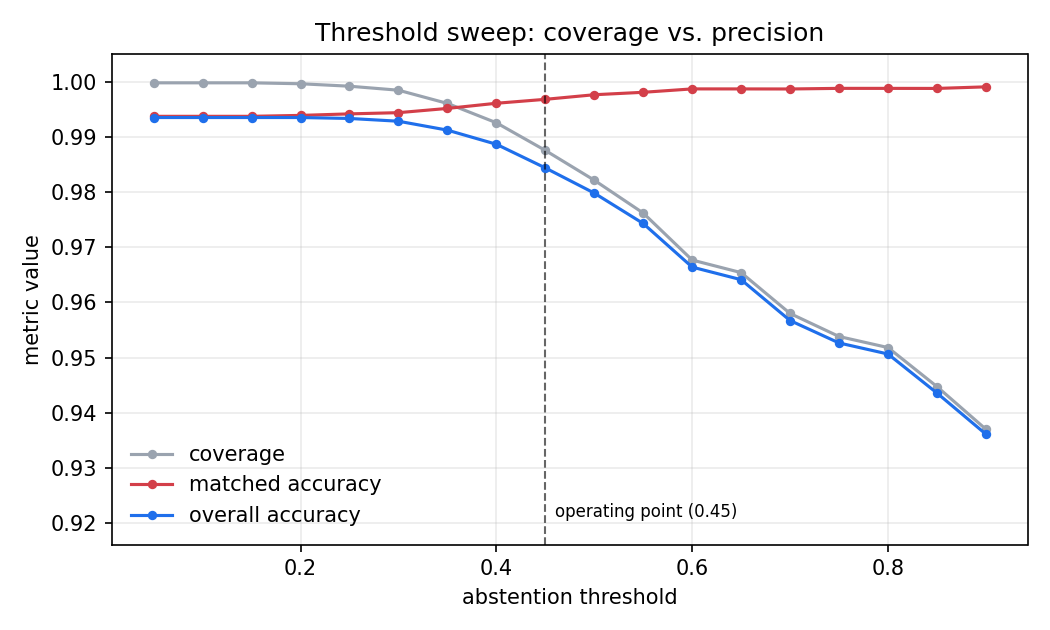
\includegraphics[width=\linewidth]{figures/threshold_sweep.png}
\caption{Coverage/precision trade-off across the abstention threshold
(hard track); the operating point $\tau{=}0.45$ is chosen from this sweep,
which the pipeline re-emits on every run.}
\label{fig:sweep}
\end{figure}

\begin{figure}[t]
\centering
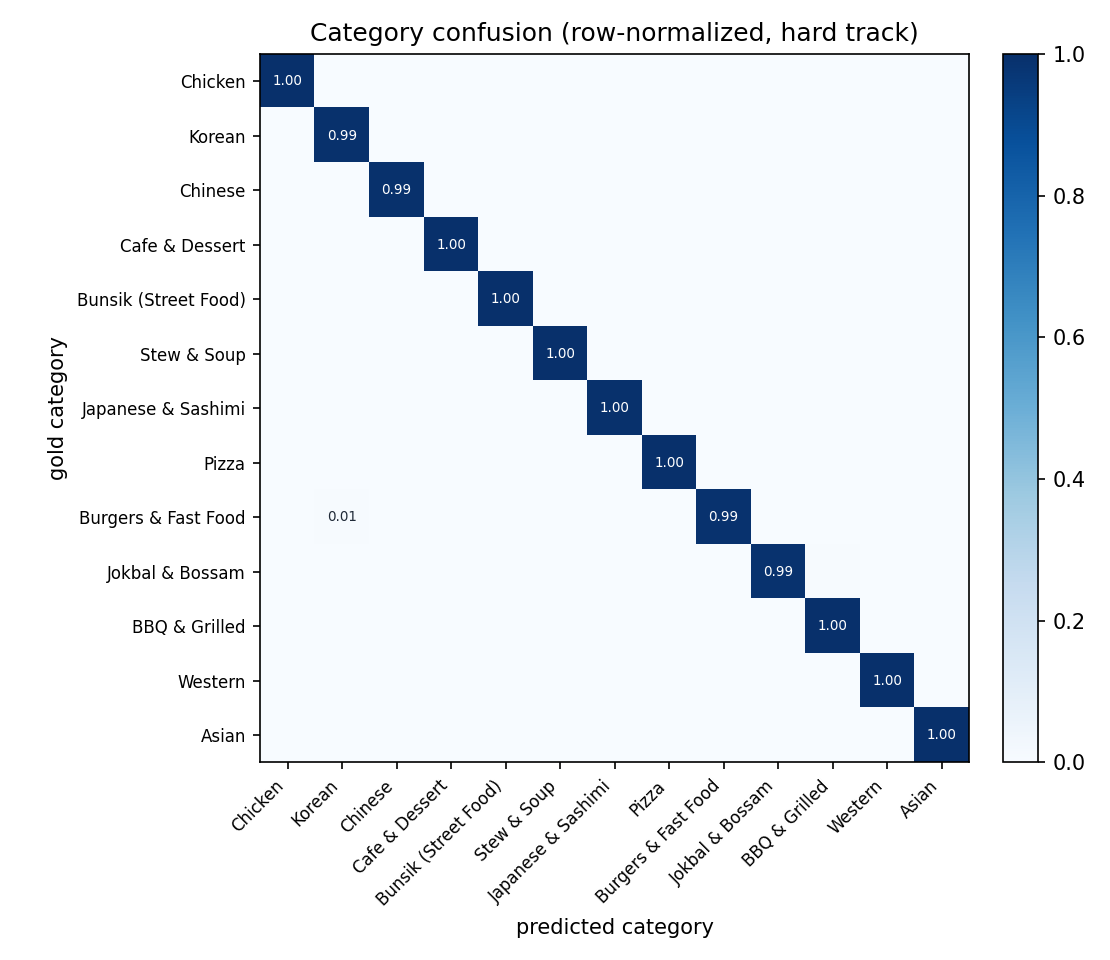
\includegraphics[width=\linewidth]{figures/confusion_matrix.png}
\caption{Row-normalized category confusion on the hard track.}
\label{fig:conf}
\end{figure}

\begin{figure}[t]
\centering
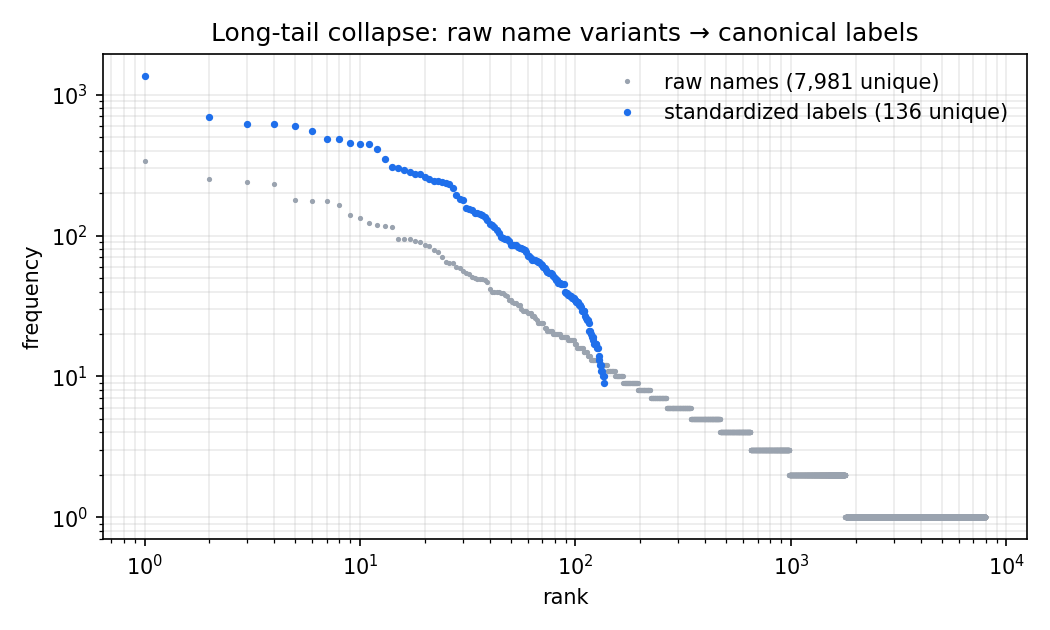
\includegraphics[width=\linewidth]{figures/long_tail.png}
\caption{Rank--frequency view of the long-tail collapse: 7{,}981 unique raw
strings map onto 136 canonical labels (hard track).}
\label{fig:tail}
\end{figure}

\textbf{Threshold behavior} (Fig.~\ref{fig:sweep}). Matched accuracy rises
and coverage falls monotonically with $\tau$, the classical reject-option
trade-off \cite{chow1970,elyaniv2010}; the sweep costs no extra similarity
computation because scores are threshold-independent.

\textbf{Efficiency and reproducibility.} A full 20k-row run completes in
roughly one second on a single core (Python 3.12), including user-dictionary
compilation. Given the seed, generation and evaluation are deterministic;
every table and figure in this paper regenerates from three commands.

\textbf{Error analysis.} Residual hard-track label errors concentrate in
(i) typos inside Latin runs that defeat the glossary after corruption and
(ii) deletions that make two labels nearly equidistant
(\mbox{크 로와상} drifting toward 크로플); the abstention mechanism converts
a majority of the latter into \unmatched{} plus a correct category rather
than a confident wrong label.

\section{Limitations}
\label{sec:limitations}

The benchmark is synthetic: although its noise model is drawn from
documented real-world modes and the hard track removes lexicon coverage as
a confound, absolute numbers remain optimistic relative to open-world
production data (unknown typo classes, OCR noise, emerging menu items).
The \texttt{benchmark\_share} weights are a design choice informed by
heterogeneous published statistics, not a market measurement, and should
not be cited as such. Code-switching recovery depends on an offline
glossary; unseen romanizations fall through to \unmatched{} (with a
category still assigned) rather than being guessed. Finally, the canonical
inventory (136 labels) is deliberately small; scaling to $10^3$ labels with
approximate-nearest-neighbor search, and adding an embedding-based third
fusion candidate under the same ablation protocol, are the natural next
steps. The original engagement's reported outcome ($\sim$20M records to
$\sim$1K labels at $\sim$95\,\% on a hand-audited sample) is provided as
motivating context only and is not reproducible from the released
artifacts.

\section{Conclusion}

\menunorm{} recasts an ad-hoc industrial standardization effort as a
reproducible research artifact: a two-level formulation that reconciles
honest abstention with total category coverage, a fusion matcher whose
benefit is demonstrated by ablation rather than asserted, a taxonomy whose
every boundary decision is sourced and logged, and a benchmark engineered to
be hard to game---closed-world ceiling made explicit, shortcut column
poisoned, typo track uncovered by any lexicon. We hope the release serves
both as a practical tool for Korean commerce text and as a template for
turning NDA-bound industrial work into verifiable science.

\begin{thebibliography}{16}\small

\bibitem{cavnar1994}
W.~B. Cavnar and J.~M. Trenkle.
\newblock N-gram-based text categorization.
\newblock In \emph{Proc.\ 3rd Annual Symposium on Document Analysis and
Information Retrieval (SDAIR)}, pages 161--175, 1994.

\bibitem{cevahir2016}
A.~Cevahir and K.~Murakami.
\newblock Large-scale multi-class and hierarchical product categorization
for an e-commerce giant.
\newblock In \emph{Proc.\ COLING}, pages 525--535, 2016.

\bibitem{chow1970}
C.~K. Chow.
\newblock On optimum recognition error and reject tradeoff.
\newblock \emph{IEEE Transactions on Information Theory}, 16(1):41--46,
1970.

\bibitem{christen2005}
P.~Christen.
\newblock Probabilistic data generation for deduplication and data linkage.
\newblock In \emph{Proc.\ IDEAL}, pages 109--116. Springer, 2005.

\bibitem{christen2012}
P.~Christen.
\newblock \emph{Data Matching: Concepts and Techniques for Record Linkage,
Entity Resolution, and Duplicate Detection}.
\newblock Springer, 2012.

\bibitem{cohen2003}
W.~W. Cohen, P.~Ravikumar, and S.~E. Fienberg.
\newblock A comparison of string distance metrics for name-matching tasks.
\newblock In \emph{Proc.\ IJCAI Workshop on Information Integration on the
Web (IIWeb)}, pages 73--78, 2003.

\bibitem{elyaniv2010}
R.~El-Yaniv and Y.~Wiener.
\newblock On the foundations of noise-free selective classification.
\newblock \emph{Journal of Machine Learning Research}, 11:1605--1641, 2010.

\bibitem{geirhos2020}
R.~Geirhos, J.-H. Jacobsen, C.~Michaelis, R.~Zemel, W.~Brendel,
M.~Bethge, and F.~A. Wichmann.
\newblock Shortcut learning in deep neural networks.
\newblock \emph{Nature Machine Intelligence}, 2:665--673, 2020.

\bibitem{hana2022}
Hana Institute of Finance.
\newblock 배달 앱 이용 현황과 메뉴 유형별 수요 특성 (Delivery-app usage
and demand characteristics by menu type). Card-payment data analysis
report, 2022.

\bibitem{kudo2004}
T.~Kudo, K.~Yamamoto, and Y.~Matsumoto.
\newblock Applying conditional random fields to Japanese morphological
analysis.
\newblock In \emph{Proc.\ EMNLP}, pages 230--237, 2004.

\bibitem{lloyd1982}
S.~P. Lloyd.
\newblock Least squares quantization in PCM.
\newblock \emph{IEEE Transactions on Information Theory}, 28(2):129--137,
1982.

\bibitem{mcnamee2004}
P.~McNamee and J.~Mayfield.
\newblock Character n-gram tokenization for European language text
retrieval.
\newblock \emph{Information Retrieval}, 7(1--2):73--97, 2004.

\bibitem{park2014}
E.~L. Park and S.~Cho.
\newblock KoNLPy: Korean natural language processing in Python.
\newblock In \emph{Proc.\ 26th Annual Conference on Human and Cognitive
Language Technology (HCLT)}, 2014.

\bibitem{pedregosa2011}
F.~Pedregosa et~al.
\newblock Scikit-learn: Machine learning in Python.
\newblock \emph{Journal of Machine Learning Research}, 12:2825--2830, 2011.

\bibitem{yogiyo}
Yogiyo partner documentation.
\newblock 요기요 카테고리 소개 (Introduction to Yogiyo categories).
\newblock \url{https://partner.yogiyo.co.kr}, accessed 2026.

\bibitem{zipf1949}
G.~K. Zipf.
\newblock \emph{Human Behavior and the Principle of Least Effort}.
\newblock Addison-Wesley, 1949.

\end{thebibliography}

\end{document}
